\subsection{Data Processing}
Nordpoolspot \cite{nordpool} provides the energy price data used by the implemented HEMS for the demand response algorithm. The dataset has two columns: \textit{starting}, which contains a timestamp denoting the price's day and hour, and \textit{energy\_market\_price}, which holds the relative price.
\begin{table}[H]
\centering
\begin{tabular}{|c|c|}
\hline
\textbf{starting} & \textbf{energy\_market\_price} \\ \hline
\end{tabular}
\caption{Representation of the dataset \textit{energy.60.csv}}
\label{tab:dataset_energy_60}
\end{table}

The actual structure of the dataset does not make it ready-to-use for a neural network model. Our goal is to forecast prices over the next 12 hours. We may train a model using prices from the previous hours, specifically, the previous 50 hours, to accomplish this. \\
One crucial step before creating the new dataset is to verify the presence of nan values and remove them if so. The Sklearn library's k-Nearest Neighbors function was used to fill in missing values. The mean value from n nearest neighbors discovered in the training set is used to impute missing values for each sample. If the qualities that neither sample lacks are similar, the samples are similar.
\begin{minted}[fontsize=\footnotesize, numbersep=-14pt, frame=lines, linenos, breaklines]{python}
    imputer = KNNImputer(n_neighbors=2, weights='uniform')
    transformed_data = pd.DataFrame(imputer.fit_transform(df[['energy_market_price']]), columns=['energy_market_price'])
\end{minted}
The imputation was done with two neighbors, and the weighting technique was uniform: all points in each neighborhood were weighted equally. We do not have to worry about outliers because the house's energy prices and consumption records have already been checked and cleaned, and our data was collected from there. \\
We can now begin constructing the dataset that will be used to train the model. To accomplish so, we developed a simple algorithm that generates a CSV file with 64 columns: a timestamp, 50 energy prices from the previous 50 hours, the current price we are looking at, and then the prices for the next 12 hours.
\begin{minted}[fontsize=\footnotesize, numbersep=-14pt, frame=lines, linenos, breaklines]{python}
    def create_dataset(energy, nn_datas):
        energy_market_price = []
        with open(energy, "r") as energy_60_file, open(nn_datas, "w") as nn_datas_file:
            reader = csv.reader(energy_60_file)
            writer = csv.writer(nn_datas_file)
            headers = ['timestamp']
            headers.extend(['energy_price_ahead_' + str(n) for n in range(50, 0, -1)])
            headers.extend(['energy_price_forward_' + str(n) for n in range(0, 13)])
            writer.writerow(headers)
            timestamp = []
            for index, row in islice(enumerate(reader), 1, None):
                energy_market_price.append(row[1])
                timestamp.append(row[0])
                if index > 62:
                    new_line = [timestamp[index - 13]]
                    new_line.extend(energy_market_price[index - 63: index])
                    writer.writerow(new_line)
\end{minted}
\subsection{The model}
\subsubsection{Definition}
Long Short Term Memory, \textbf{LSTM}, is a type of recurrent neural network that can handle long-term dependencies. We decided to use the LSTM model because of its ability to preserve long-term dependencies. Furthermore, it also reduces the problem of the vanishing gradient along the temporal line. \\ Its architecture is similar to an RNN cell. In an RNN, the structure is a chain of repeating simple modules of a neural network.

\begin{figure}[H]
    \centering
    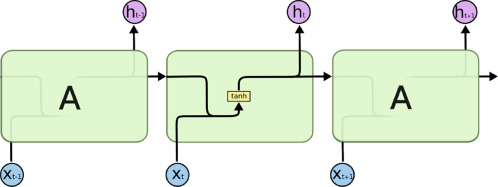
\includegraphics[width=0.9\textwidth]{LSTM immagini/RNN.jpg}
    \caption{RNN architecture}
\end{figure}

In an LSTM, the repeating module has a different structure. It is composed of four interacting neural network layers.

\begin{figure}[H]
    \centering
    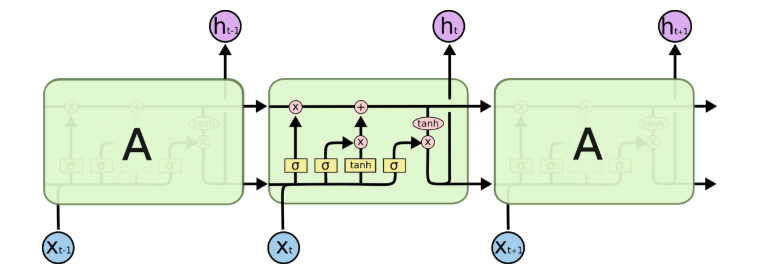
\includegraphics[width=\textwidth]{LSTM immagini/LSTM.png}
    \caption{LSTM architecture}
\end{figure}
Inside an LSTM cell, we can distinguish between:
\begin{itemize}
    \item \textbf{Cell State}, which reduces the problem of short memory in an RNN. It maintains a vector $C_t$ which dimension is the same as the hidden state $h_t$. Inside the cell state, the information can be forgotten using the \textbf{Forget Operator (X)} but also added using the \textbf{Input (+) Operator}.
    
    \begin{figure}[H]
        \centering
        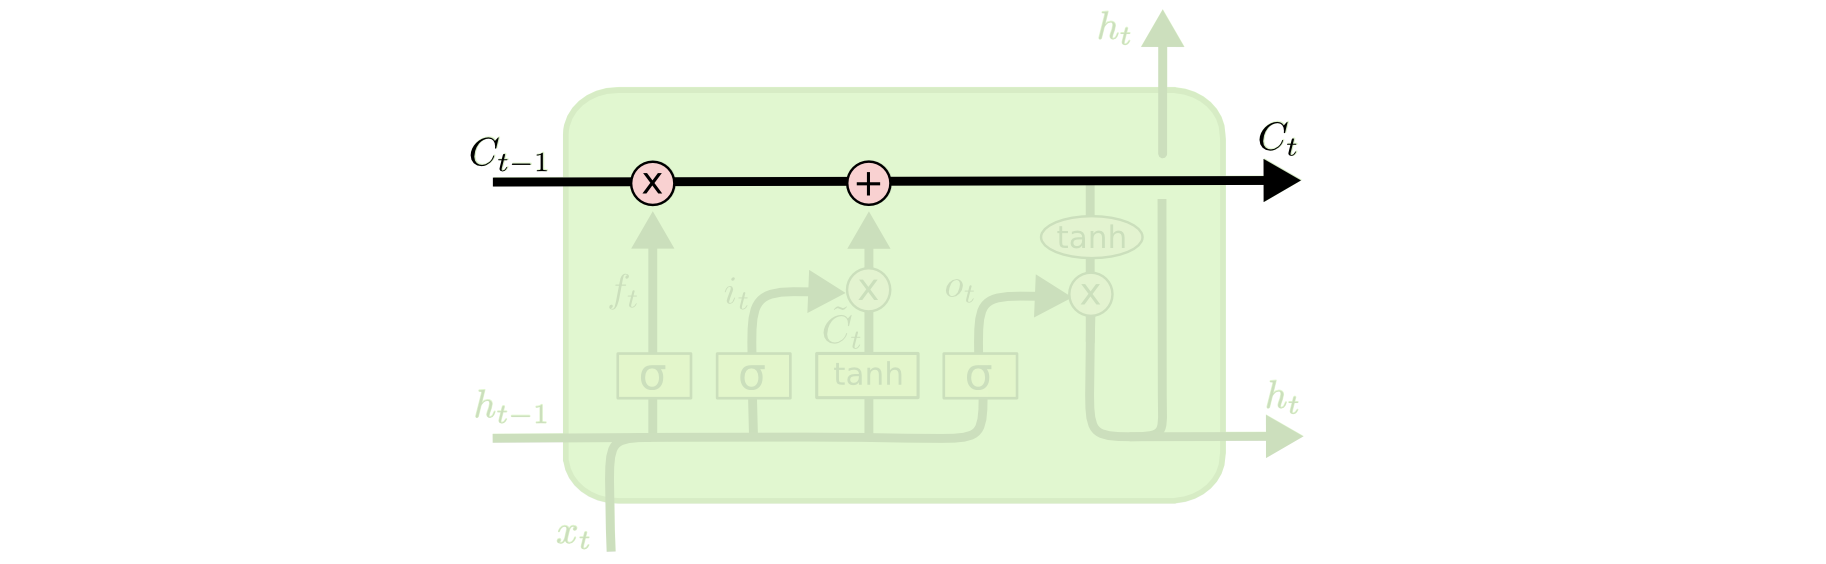
\includegraphics[width=0.8\textwidth]{LSTM immagini/cell state.png}
        \caption{Cell State of an LSTM}
    \end{figure}
    
    \item \textbf{Forget Gate} is a sigmoid layer that decides what should be forgotten about the previous state. It takes $h_{t-1}$ and $x_t$ as input and outputs a value between 0 and 1 where 0 is \textit{completely keep this value} and 1 is \textit{completely forget about this value}.
    \begin{figure}[H]
        \centering
        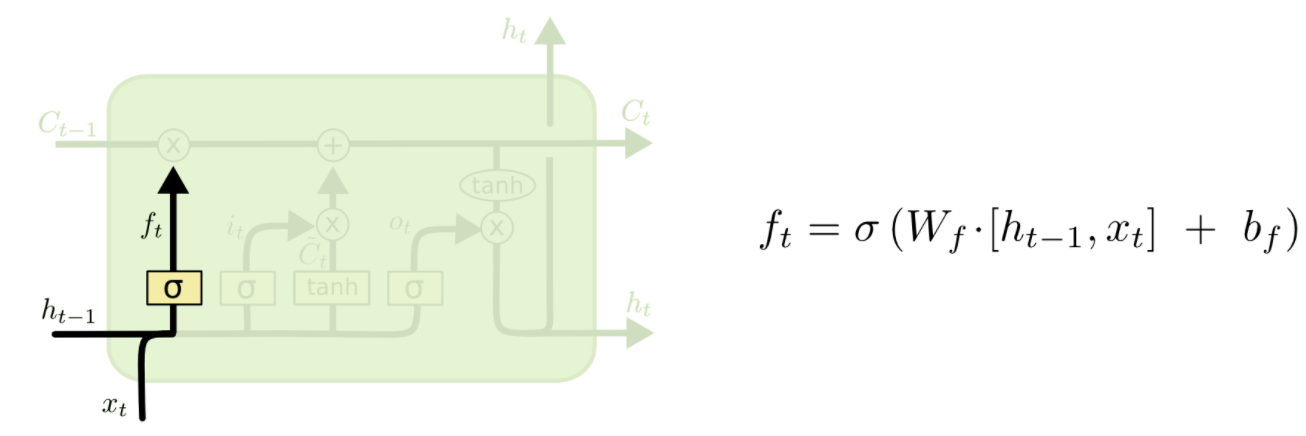
\includegraphics[width=0.8\textwidth]{LSTM immagini/forget gate.png}
        \caption{Forget Gate of a LSTM cell}
    \end{figure}
    
    \item \textbf{Input Gate} comprises a sigmoid layer that decides which values to update and a tahn layer that determines the amount to add/subtract from these values.
    
    \begin{figure}[H]
        \centering
        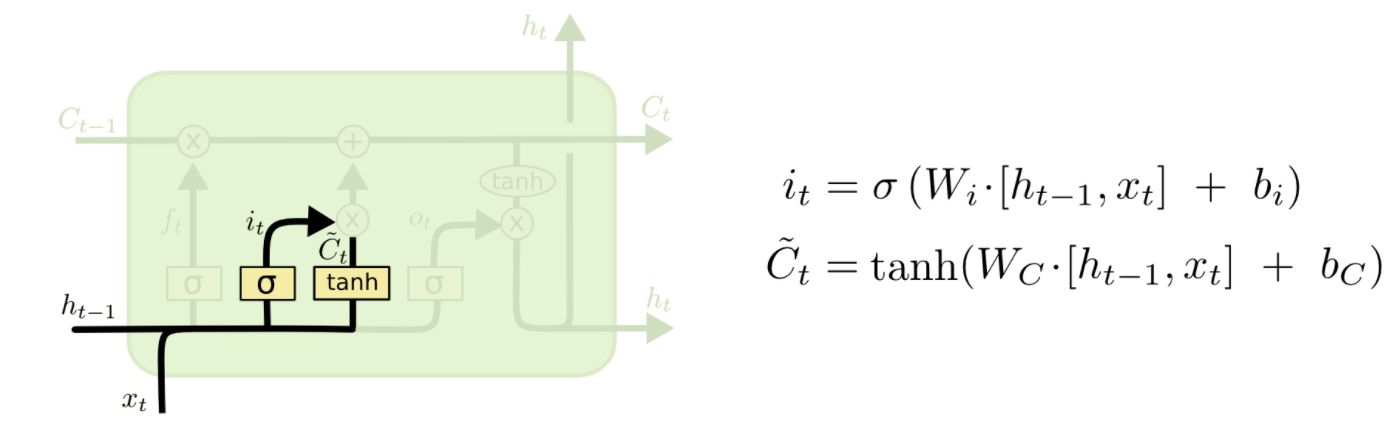
\includegraphics[width=0.8\textwidth]{LSTM immagini/input gate.png}
        \caption{Input Gate of a LSTM cell}
    \end{figure}
    
    \item \textbf{Output Gate} decides what goes to the next layer and the next state based on our cell state, which was scaled to [-1,1] using the tahn. The output is computed using the sigmoid function between the scaled cell state output and the current hidden state.
    
    \begin{figure}[H]
        \centering
        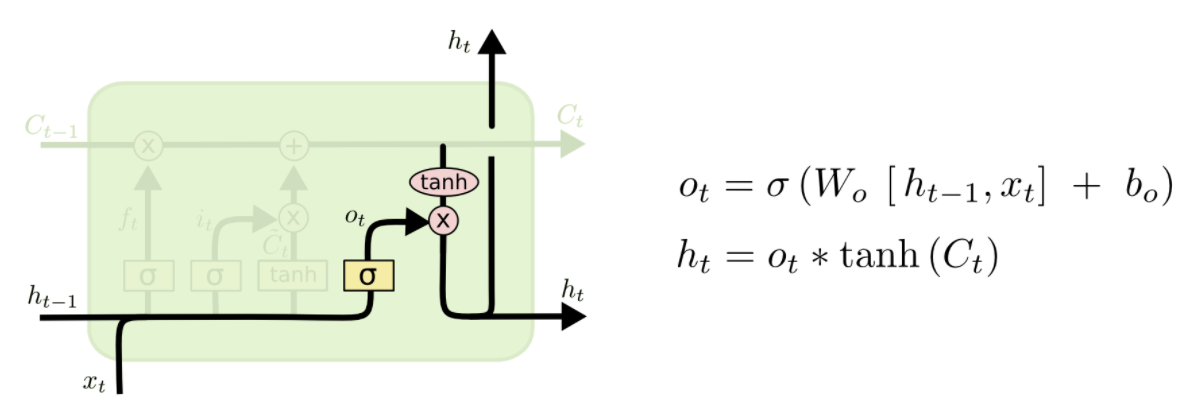
\includegraphics[width=0.8\textwidth]{LSTM immagini/output gate.png}
        \caption{Output Gate of a LSTM cell}
    \end{figure}
\end{itemize}
\textit{Nevertheless, how is the cell state updated?}  We multiply the old state $C_{t-1}$ by $f_t$, the output of the Forget Gate. Then we add $i_t * \tilde{C}_i$, which was the output of the Input Gate. We obtain the new cell state $C_t$.

\begin{figure}[H]
    \centering
    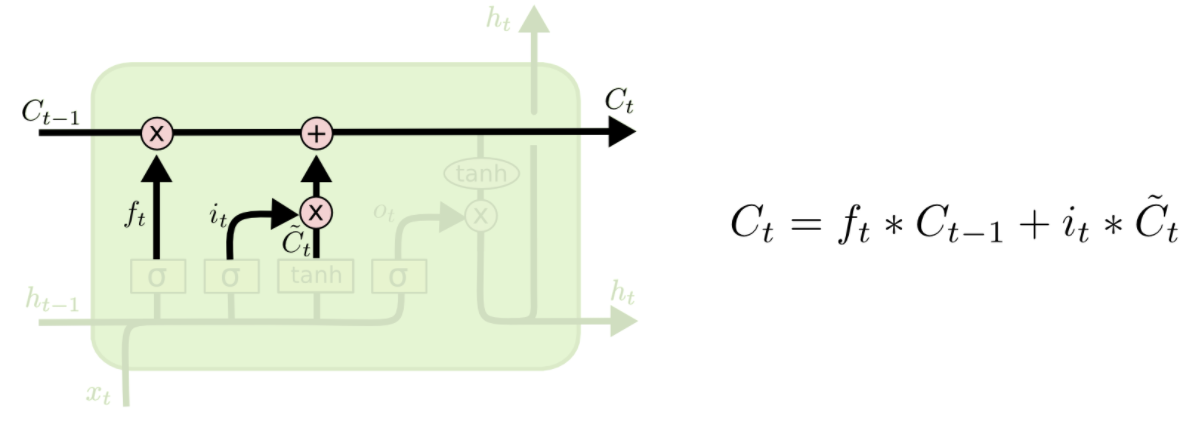
\includegraphics[width=0.8\textwidth]{LSTM immagini/update cell state.png}
    \caption{Updating the cell state in a LSTM}
\end{figure}
The applications of an LSTM are countless: we used it in time series prediction for which is most suited.
\subsubsection{Implementation}
We choose Keras as a library to implement our model. \textit{Keras} is an open-source software library that provides a Python interface for artificial neural networks. It acts as an interface for the Tensorflow library.
Using Keras, we were able to define each layer of our LSTM model in the following way:

\begin{minted}[fontsize=\footnotesize, numbersep=-14pt, frame=lines, linenos, breaklines]{python}
    model = Sequential()
    model.add(LSTM(units=50, return_sequences=True, input_shape=(50, 1)))
    model.add(Dropout(0.5))
    model.add(LSTM(units=50))
    model.add(Dropout(0.5))
    model.add(Dense(12))
    model.compile(optimizer='adam', loss="mse", metrics=['mse', 'mae', 'mape'])
\end{minted}

The first layer incorporates 50 units and takes 50 features as input. Those features represent the prices of the energy for the previous 50 hours. A dropout layer was added after each LSTM layer to avoid over-fitting. The hidden layer is composed of an LSTM layer with 50 units. The last layer is a Dense one with 12 outputs for the prices of the following 12 hours to be predicted. \\
The model was compiled using the \textit{Adam Optimizer}, a stochastic gradient descent method that is based on adaptive estimation of first-order and second-order moments. The function to minimize is the Mean Square Error, the average squared difference between the estimated values and the actual value. The compile function will also calculate the Mean Absolute Error, the distance between the predicted and actual value, and the Mean Absolute Percentage Error. This model is a relative-simple implementation used in the first phases of the research (it will be changed afterward using hyper-parameter search) to understand if the LSTM is a valid prediction model for our data.
\subsubsection{Training and Testing}
For the training and testing part, the dataset was split into train (70\%) and testing (30\%), without shuffling. Our dataset is a strictly correlated time series, so shuffling the dataset would have meant losing this connection. \\ 
Each set was then scaled in the range [0,1] using the MinMaxScaler provided by the Sklearn library. Scaling the dataset makes it easy for the model to learn and understand the problem.
\begin{minted}[fontsize=\footnotesize, numbersep=-14pt, frame=lines, linenos, breaklines]{python}
    scaler = MinMaxScaler(feature_range=(0, 1))
    
    scaled_x = (pd.DataFrame( df['timestamp']).join(pd.DataFrame(scaler.fit_transform(x)))).to_numpy()
    scaled_y = scaler.fit_transform(y)
    
    x_train, x_test, y_train, y_test = train_test_split(scaled_x, scaled_y, shuffle=False, random_state=42, test_size=0.3)
\end{minted}

The model was trained using 20 epochs and a batch size of 32. Additionally, it was given the size of the \textit{validation dataset} (20\% of training dataset). The validation dataset can provide some helpful information to optimize hyperparameters. It can also be an indicator of overfitting.

\begin{minted}[fontsize=\footnotesize, numbersep=-14pt, frame=lines, linenos, breaklines]{python}
    model.fit(x_train[:, 1:].astype('float64'), y_train, epochs=20, batch_size=32, verbose=2, validation_split=0.2, callbacks=[callback])
\end{minted}

After the training, we can plot the \textit{loss} and the \textit{validation loss} through the epochs:

\begin{figure}[H]
    \centering
    \includesvg[width=\textwidth]{LSTM immagini/baseline_loss.svg}
    \caption{Loss and Validation Loss through the epochs}
    \label{lte1}
\end{figure}

As we can see from \autoref{lte1}, the \textit{loss} decreases as the epochs increases. In this case, the validation loss is lower than the training loss: it indicates that the validation dataset is easier for the model to predict than the training dataset. The model was then used to predict the price for the 12 hours ahead of using the custom function. The result was saved unscaled.
\subsubsection{Evaluation}
Using the test set, we were able to see graphically how much our predictions differ from the ground truth. 
\begin{figure}[H]
    \centering
    \includesvg[width=0.8\textwidth]{LSTM immagini/baseline_model.svg}
    \caption{Comparison between the real values and the predicted values}
    \label{lte2}
\end{figure}
As we can see from \autoref{lte2}, the prediction does not strictly follow the actual values. They are concentrated in one point, between 0.5 and 0.6. This means that the LSTM nearly always predicts the same value. However, if we analyze \autoref{lte1}, the mean squared error used as loss function in the model is decreasing. \\
As we said before, since this is a time series strictly correlated, we cannot do k-fold cross-validation to obtain a more general evaluation. Another evaluation method used on every model is the Root Mean Squared Error: a frequently used measure of the differences between predicted and actual values.
\begin{minted}[fontsize=\footnotesize, numbersep=-14pt, frame=lines, linenos, breaklines]{python}
    rms = np.sqrt(mean_squared_error(y_test, preds))
\end{minted}
The result for the first model was 0.059002225233545286. The lower the RMSE, the better the model is able to fit a dataset. In conclusion, the LSTM model is a good predictor and an ideal choice to solve our problem.
\subsubsection{Hyper-parameter tuning}
Not yet satisfied with the result, we decided to use the Keras Tuner framework to perform a better hyperparameter search to create a model with better performance. The KerasTuner is an easy hyperparameter optimization framework that finds the best hyperparameter for a given model. It provides many different algorithms to conduct the hyperparameter search: we used the Hyperband. \\
The first step was to define which parameters could the tuner set:
\begin{itemize}
    \item The number of units in the first LSTM layer
    \item The Dropout rate in the first Dropout layer
    \item Number of additional LSTM layer with their units and additional Dropout layer with their rate
    \item The activation function (relu or sigmoid) in the last Dense layer
    \item The learning rate of the model
\end{itemize}
\begin{minted}[fontsize=\footnotesize, numbersep=-14pt, frame=lines, linenos, breaklines]{python}
    def hypermodel_builder(hp):
    
        model = Sequential()
        model.add(LSTM(units=hp.Int('units_first_layer', min_value=32, max_value=512, step=32), return_sequences=True, input_shape=(50, 1)))
    
        model.add(Dropout(hp.Float('Dropout_rate_first_layer', min_value=0.1, max_value=0.5, step=0.1)))
    
        for i in range(hp.Int('n_additional_layers', 1, 4)):
            model.add(LSTM(units=hp.Int('units_add_layer', min_value=32, max_value=512, step=32), return_sequences=True))
            
            for j in range(hp.Int('n_additional_dropout_layers', 0, 1)):
                model.add(Dropout(hp.Float('Dropout_rate_add_layer', min_value=0.1, max_value=0.5, step=0.1)))
    
        model.add(Flatten())
    
        model.add(Dense(12, activation=hp.Choice('dense_activation', values=['relu', 'sigmoid'], default='relu')))
    
        model.compile(optimizer=Adam(lr=hp.Choice('learning_rate', values=[1e-2, 1e-3, 1e-4])), loss=['mean_squared_error'], metrics=['mse', 'mae', 'mape', RootMeanSquaredError()])
        
        return model
\end{minted}
Once that we've defined the model, we can run the tuner. The KerasTuner takes as input: 
\begin{itemize}
    \item The model
    \item The objective function to minimize
    \item The maximum number of epochs to be tried
    \item A factor used to calculate the number of trials 
    \item The directory in which to save the results
\end{itemize}
\begin{minted}[fontsize=\footnotesize, numbersep=-14pt, frame=lines, linenos, breaklines]{python}
    tuner = kt.Hyperband(hypermodel_builder, kt.Objective("root_mean_squared_error", direction="min"), max_epochs=30, factor=3, directory='output', project_name='LSTM 3.0')
\end{minted}
Now everything is ready to start the tuner. We have added a callback to stop the tuner when the validation loss increases for three models in a row.
\begin{minted}[fontsize=\footnotesize, numbersep=-14pt, frame=lines, linenos, breaklines]{python}
    callback = EarlyStopping(monitor='val_loss', patience=3, restore_best_weights=True)
    
    tuner.search(x_train[:, 1:].astype('float64'), y_train, validation_split=0.2, callbacks=[callback])
\end{minted}

The trials went on for 3 hours; each trial lasted from a few seconds to 10 minutes. In the end, the best model was chosen with these characteristics:
\begin{itemize}
    \item 384 units in the first LSTM layer
    \item 0.30000000000000004 dropout rate for the first Dropout layer
    \item 2 additional LSTM layer with 320 units
    \item 0 additional Dropout layer
    \item The sigmoid function as activation function
    \item 0.001 learning rate with the Adam optimizer
    \item 30 epochs
\end{itemize}
Once the model is defined, we can train it using the training dataset and plot the predictions against the actual values:
\begin{figure}[H]
    \centering
    \includesvg[width=0.8\textwidth]{LSTM immagini/hyper_model.svg}
    \caption{Comparison between the real values and the predicted values}
    \label{fig:hyper_loss}
\end{figure}
As we can see from \autoref{fig:hyper_loss}, the newly trained model is much more accurate in its prediction than the previous one. The next hour energy price is more precise than the following hours: we can clearly say that the accuracy decreases over time. This phenomenon is expected and also experienced in the previous model. \\
Also for this model, we can plot the \textit{loss} and the \textit{validation loss} through the epochs:
\begin{figure}[H]
    \centering
    \includesvg[width=\textwidth]{LSTM immagini/hypermodel_loss.svg}
    \caption{Loss and Validation Loss through the epochs using the hypermodel}
    \label{fig:hyper_rmse}
\end{figure}
As shown in \autoref{fig:hyper_rmse}, there are some spikes in the validation loss.These spikes are standard and happen when the validation dataset is too small. However, the small size of the overall dataset does not allow us to use a more extensive validation dataset.  \\
The plot also shows that the loss decreases through the epochs, indicating that the model is learning. The RMSE for this model was 0.042919002838567366, slightly lower than the previous model. \\ 
As \autoref{Tab:summary_table} displays, the performance of the hyper model is slightly better than the performance of the base model.  The tuner was able to find a model whose loss is lower than the one we have constructed before. Consequently, this model is more promising than the previous one, and its predictions will be used to perform the reinforcement learning stage. 
\begin{table}[h!]
\centering
\caption{Summary Table}
\label{Tab:summary_table}
\begin{tabular}{|c|c|c|}
\hline
                                                                                   & \textbf{Base Model} & \textbf{Hyper Model} \\ \hline
\textbf{\begin{tabular}[c]{@{}c@{}}Root Mean \\ Squared Error\end{tabular}}        & 0.059002            & 0.042919             \\ \hline
\textbf{Mean  Squared Error}                                                       & 0.003481            & 0.001842             \\ \hline
\textbf{Mean Absolute Error}                                                       & 0.040115            & 0.029098             \\ \hline
\textbf{\begin{tabular}[c]{@{}c@{}}Mean Absolute \\ Percentage Error\end{tabular}} & 0.070619            & 0.052231             \\ \hline
\end{tabular}

\end{table}